\subsection{Dalvik Executionable File Format} \label{subsection:android-dex}
%START TEXT INPUT
Android applications deliver their code in \gls{dex} bytecode.
Applications on Android are executed by the \gls{dvm} in \gls{dex} bytecode.
It can be compared to Java bytecode except some differences.
While the Java \gls{vm} is stack-based the \gls{dvm} is register-based, this circumstances have influence on the code.
The Java bytecode is actually more compact than dex since it uses 8bit constants \gls{dex} which has instructions of 16bit multiples.

The bytecode is more suited to run on the ARM architecture since it supports direct mapping from dex registers to the registers of the ARM processor.
Registers in \gls{dex} bytecode are 32bits wide and store values such as integers or float values.
In case there are 64bit values, adjacent registers are used to store it.
The \gls{dex} bytecode supports 218 valid opcodes which have a dest-sort ordering for its arguments.
The instructions refer to indexes in pools.
\begin{figure}[h]
    \centering
    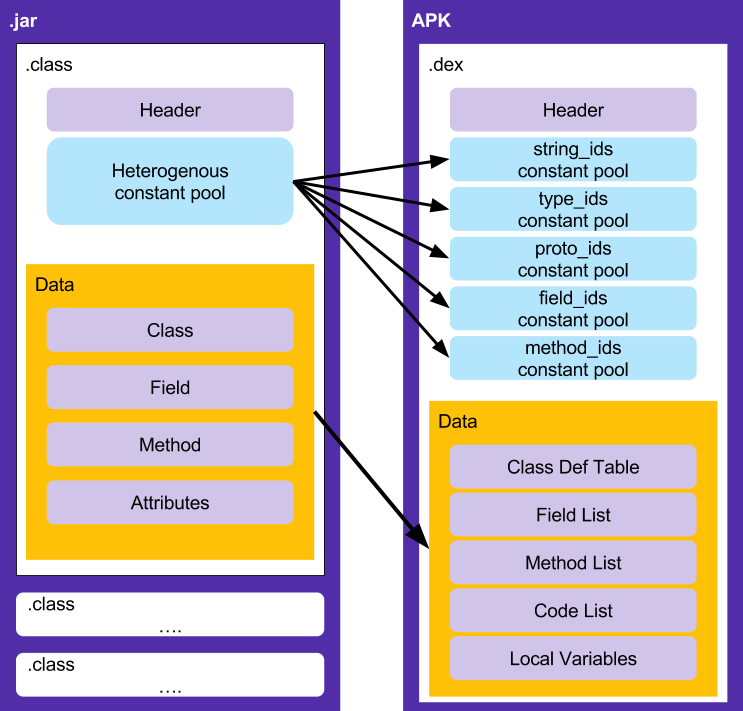
\includegraphics[width=0.5\textwidth]{data/java.png}
    \caption{\gls{jar} to \gls{apk} transformation \cite{googleDalvik}}
    \label{fig:java}
\end{figure}

\begin{figure}[h]
    \centering
    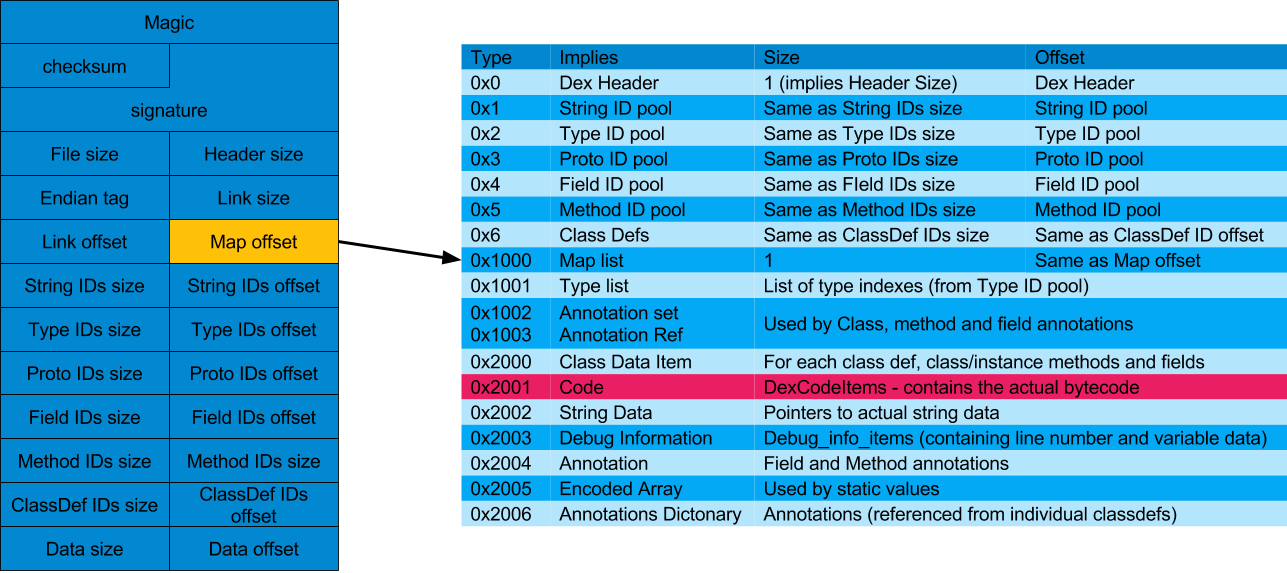
\includegraphics[width=0.8\textwidth]{data/dex.png}
    \caption{\gls{dex} file format \cite{andevconDalvikART}}
    \label{fig:dex}
\end{figure}


The applications for Android are written using the Java programming language.
The process can be seen in figure~\ref{fig:apk}.
The first steps are similar to the build process of Java applications.
In the first step the Java files are compiled
The Java files are compiled into \gls{classg} files by the Java compiler
step 1:  Java files which will be compiled into \gls{classg} files by a Java Compiler,  similar to a Java program build process, class files contain Java bytecode representing the compiled application, optional step apply a Java Obfuscator\newline

When compiling, the application is first compiled to \gls{jar} file using the Java compiler javac.
The jar contains the \gls{classg}, which are the Java classes in bytecode, as well as the heterogenous constant pool.
In order to create the dex file, which is called classes.dex, dx is used on the \gls{jar} file.
Dx compiles the Java bytecode to \gls{dex} byte code and sorts string, type and method from the heterogenous pool in seperated pools and removes dublicates.
This results in figure~\ref{fig:java}
This is most effective for string and this action results in a memory footprint which is up to 44\% lower than the one of the \gls{jar}.
The result is that the \gls{dex} file has significant more references than the \gls{jar} file.
The \gls{dex} file is stored as classes.\cite{ehringerDalvik}

Like Java bytecode \gls{dex} bytecode allows easy decompilation to Java.
Also since the bytecode is in contrast to other architectures pretty simple and only in rare cases protection is applied, it is an easy target for reverse engineering.

Since \gls{dex} bytecode supports optimization, improvements for the underlying architecture can be applied to the bytecode upon installation.
The resulting \gls{dex} file is called \gls{odex}.
The optimizations are executed by a programm called dexopt which is part of the Android plattform.
For the \gls{dvm} it makes no difference whether \gls{dex} or \gls{odex} files are executed, except speed improvements.
%



%AUFBAU DEX
%DVM is register based. Registers are considered 32 bits wide to store values such as integers or floating point numbers. Adjacent register pairs are used to store 64-bit values\newline
%dest-then-source ordering for its arguments\newline
%there are 218 used valid opcodes in Dalvik bytecode -see- QUELLE \newline

%Due to its simplicity over bytecode for other architectures as well as the little protection applied in practice, Dalvik bytecode is currently an easy target for the reverse engineer.


%Each .class file has its own heterogeneous constant pool which may contain duplicating data, BEISPIEL, memory efficiency of a .dex file comes primarily from the type-specific constant pools used to store the data, BEISPIEL,\newline
%significantly more references within a .dex file compared to a .class file\cite{ehringerDalvik}\newline
%compression as efficiently as up to 44 percent of the size of an equivalent .jar archive\cite{ehringerDalvik}\newline
%hier noch einfach dex, später erst opcode nennen, the exact dex format will be explained in 2.4.2\newline

%\cite{kovachevaMaster} \cite{ehringerDalvik}
%

%
%dx utility converts multilple class files to classes.dex, java bytecode is converted to dex bytecode, dex instructions 16bit mltiples, java 8bit
%constant, string,type and method pools are merged, significant savings for strings, types and methods in multiple calsses
%overall memory footprint diminished by about 50%
%dex file format specified in android dcomentation -see- SOURCE\newline

%dex instructions refer to indexes (in pools)\newline
%dex bytecode is striktly similar to java bytecode, allows for ease de-/re %compilation back and forth to/from java\newline

%dex vs java\newline
%java vm is stack based, dex is register based
%java bytecode is actually more compact than dex
%dex bytecode is more suited to arm architectures, mapping from dex registers to arm registers
%dex supports bytecode optimizations, java no, apk's calsses.dex are optimized before install, on device\newline
%\cite{andevconDalvikART}
%

%AUFBAU DALVIK BYTECODE\newline
%The program code of an Android application is delivered in form of Dalvik bytecode\newline
%It will be executed by the Dalvik Virtual Machine and is comparable to Java bytecode.
%So there is a separate optimizing step while installing an application, where the bytecode gets optimized for the underlaying architecture. The optimized form is also called ”odex”. The optimization is done by a program called ”dexopt” which is part of the Android platform. The DVM can execute optimized as well as not optimized Dalvik bytecode\newline

%.dex file
%The Dalvik bytecode consists of opcodes and is thus hard to read for humans. The Cracking Tool has to modify the opcodes in order to alter the behaviour of the application. Since it is directly read by the Dalvik virtual machine, it is the single point of truth.

%.odex file
%Dalvik bytecode of an application is normally not optimized, because it is executed by a DVM which can run under different architectures\newline
